\section{Założenia techniczne}
\label{sec:zalozenia_techniczne}

Ze względu na charakter aplikacji, jakim jest edukacyjna gra komputerowa,
opierająca się w dużym stopniu na renderowaniu grafiki,
do wykonania projektu wybrano silnik Unity w wersji 6000.0.25f1.
Z wielu zalet silnika Unity, kluczowe dla niniejszego projektu są:

\begin{citemize}
    \item Wsparcie dla wielu platform --
    Unity pozwala na tworzenie aplikacji na wiele platform jednocześnie, w tym przede wszystkim na systemy Windows, Linux oraz macOS.
    \item Prostota tworzenia aplikacji graficznych --
    Unity oferuje wiele narzędzi, które ułatwiają tworzenie interaktywnych aplikacji graficznych,
    dzięki czemu można skupić się na tworzeniu mechanik gry.
    \item Szerokie wsparcie --
    Unity posiada rozbudowaną dokumentację~\cite{unity_docs},
    aktywne forum~\cite{unity_forum} oraz wiele darmowych zasobów,.
\end{citemize}

Unity korzysta z języka C\#, opartego o paradygmat programowania obiektowego (ang. OOP — Object-Oriented Programming),
polegający na tworzeniu obiektów na podstawie abstrakcji klas, a także innych obiektów~\cite{nygaard1986basic}.
Pozwala to na tworzenie wielu obiektów o podobnych cechach, co ułatwia pisanie kodu oraz jego późniejsze utrzymanie.\\

\subsection{Architektura programu}
\label{subsec:architektura_programu}

Aby zapewnić modularność oraz separację elementów aplikacji,
wykorzystano odpowiednio zaadaptowana architekturę MVVM (Model-View-ViewModel).
Polega ona na podziale na trzy główne części: model, widok oraz widok-model.
Funkcje każdego z nich opisano w tab.~\ref{tab:mvvm}.

\begin{table}[h]
    \centering
    \caption[Opis funkcji poszczególnych elementów architektury MVVM.]
    {Opis funkcji poszczególnych elementów architektury MVVM, źródło:~\cite{mvvm}.}
    \label{tab:mvvm}
    \begin{tabular}{|c|p{0.6\textwidth}|}
        \hline
        Element & Opis \\
        \hline
        \hline
        Widok & Odpowiada za prezentację danych oraz interakcję z użytkownikiem. \\
        \hline
        Widok-model & Odpowiada za przekazywanie danych pomiędzy modelem a widokiem. \\
        \hline
        Model & Odpowiada za przechowywanie danych oraz logikę danego komponentu programu. \\
        \hline
    \end{tabular}
\end{table}

%Tak jak pierwotnie w architekturze MVVM,
%widok odpowiada za prezentację danych oraz interakcję z użytkownikiem.
%Przy czym po adaptacji widok-model odpowiada za nie tylko przekazywanie danych nie tylko między modelem a widokiem,
%ale również pomiędzy innymi częściami aplikacji jako menedżer danego systemu aplikacji.
%Sam model natomiast składa się z wielu komponentów, które przechowują dane oraz logikę danego komponentu aplikacji.
W przypadku większych projektów model ten jest stosowany do większości komponentów składających się na aplikację.
Widok-model w tej sytuacji odpowiada za przekazywanie danych nie tylko między modelem a widokiem,
ale również pomiędzy innymi częściami aplikacji jako menedżer danego systemu aplikacji.
W przypadku opracowywanej aplikacji można wyróżnić trzy główne systemy dotyczące innych aspektów programu:

\begin{citemize}
    \item System zarządzania progresem gry, odpowiadający za kontrolę przebiegu gry,
    a także punktację oraz weryfikację poziomów,
    \item Narzędzia do rysowania i edycji, wybieranie ich oraz kontrola ich działania,
    \item System zarządzania rysowanym schematem,
    odpowiadający za renderowanie warstw i przechowywanie informacji o nich
    oraz kontrolujący ich widok czy połączenia, na jakie się składają,
    \item System zapisu, odpowiadający za zapis i odczyt stanu gry.
\end{citemize}

%zarządzanie progresem gry, narzędzia do rysowania i edycji, system zarządzania rysowanym schematem, oraz system zapisu.
Odstępstwem od architektury MVVM jest natomiast potrzeba bezpośredniej interakcji pomiędzy użytkownikiem,
a narzędziami ze względu na różnorodność interakcji co przekłada się także na mniej skomplikowany kod.\\
Zarys architektury programu przedstawiono na rys.~\ref{fig:architektura}.

\begin{figure}[h!]
    \centering
    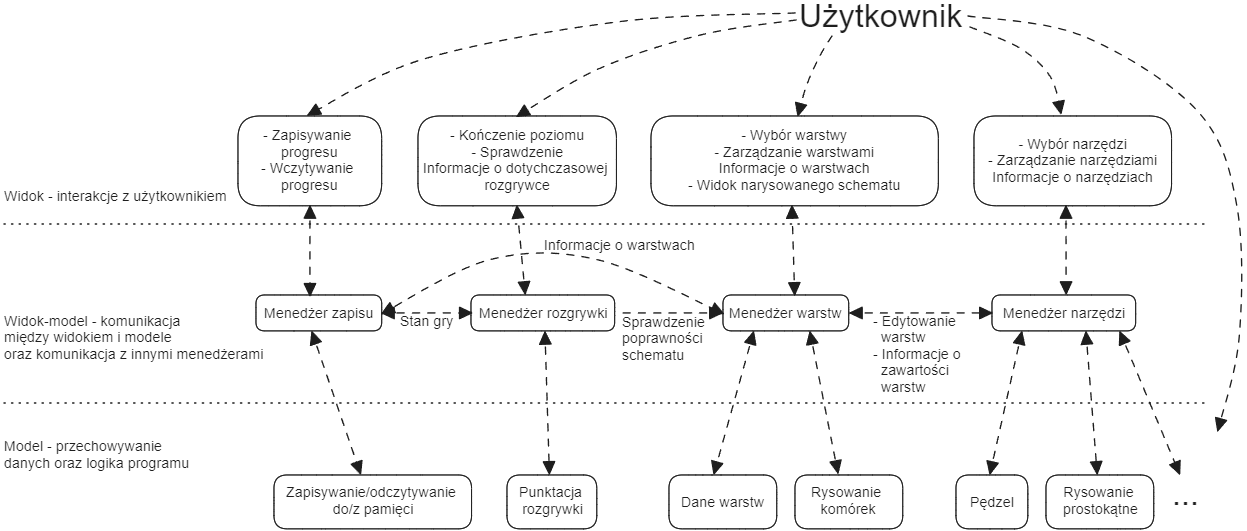
\includegraphics[width=\textwidth]{chapters/chapter3/rys/arch}
    \caption[Architektura programu.]{Architektura programu, źródło: opracowanie własne.}
    \label{fig:architektura}
\end{figure}

\subsection{Wykorzystanie funkcji Unity oraz paczek zasobów}
\label{subsec:zasoby}

Prócz podstawowego skryptu, na jakim bazuje Unity, czyli \textit{MonoBehaviour},
wykorzystano także \textit{ScriptableObject}.
Jest to klasa, która pozwala na tworzenie obiektów, które mogą przechowywać,
a nawet wykonywać prostą logikę dane poza pracą programu~\cite{unity_csharp, scriptable_docs}.
%Pozwala to na szczególną modularność dzięki możliwości wcześniejszego zdefiniowania danych zawartych w obiekcie
%i co mają one robić, a następnie tworzenie obiektów na ich podstawie.
Działanie SO jest zbliżone do klas i obiektów w OOP,
przy czym SO jest wykorzystywany przede wszystkim w edytorze Unity.
Dzięki temu można wcześniej zdefiniować jaki rodzaj danych powinien przechowywać dany typ obiektu,
a następnie tworzyć na ich podstawie konkretne obiekty, których dane można zmieniać w edytorze.
Zostało to w szczególności wykorzystane w systemach zarządzania, rysowanym schematem
i narzędziami do rysowania i edycji.\\
%W przypadku schematu SO przechowuje informacje o tym jak powinny wyglądać i zachowywać się warstwy,
%natomiast do narzędzi SO zostały wykorzystane jako konfiguracje 
\indent 
